\FloatBarrier
\section{Data}
\label{sec:data}

This section describes the construction of the dataset used for all experiments in this thesis. The primary source is the Sloan Digital Sky Survey (SDSS) Data Release 19 (DR19)~\cite{sdss_dr19}, which contains approximately seven million optical and infrared spectra. The raw release is heavily imbalanced and includes noisy observations that can impair the training of sensitive models. Therefore, a curated subset was constructed specifically for deep learning and quantum machine learning workflows.

\subsection{Dataset Construction}
\label{sec:dataset_construction}

To obtain high-quality inputs, all SDSS DR19 queries were filtered to exclude observations with a redshift warning (\texttt{ZWARNING > 0}). This step removes spectra with unreliable redshift estimates or instrumental artefacts.

The SDSS taxonomy assigns each spectrum a primary class (STAR, GALAXY, or QSO) and a more specific subclass. In raw form, this taxonomy yields over one hundred distinct subclass combinations, many of which are physically similar or severely underrepresented. To obtain a robust classification target, a systematic subclass merging was applied. Similar subclasses were collapsed into broader categories - for example, specific luminosity classes such as B3II and B3V were merged into a single B3 class. This increased the sample density per class while preserving fundamental physical distinctions.

After merging, strict minimum and maximum sample thresholds were enforced to mitigate extreme class imbalances. Any class with fewer than 250 valid samples was removed, which eliminated nine severely underrepresented classes. To prevent the largest classes (e.g., normal galaxies or quasars) from dominating the loss landscape, data acquisition was initially capped at a maximum of 25,000 samples per class. This ceiling provides sufficient data for various experimental subsets while maintaining a manageable overall dataset size. For the primary baseline experiment, the majority classes were further downsampled to a cap of 5,000 samples each.

The final filtered dataset comprises approximately 645'000 spectra distributed across 62 merged classes. This size provides a rigorous testbed for classical architectures while allowing targeted subsets for the parameter-constrained quantum experiments. Figure~\ref{fig:spectra_examples} shows representative examples of four distinct spectral classes.

\begin{figure}[htbp]
    \centering
    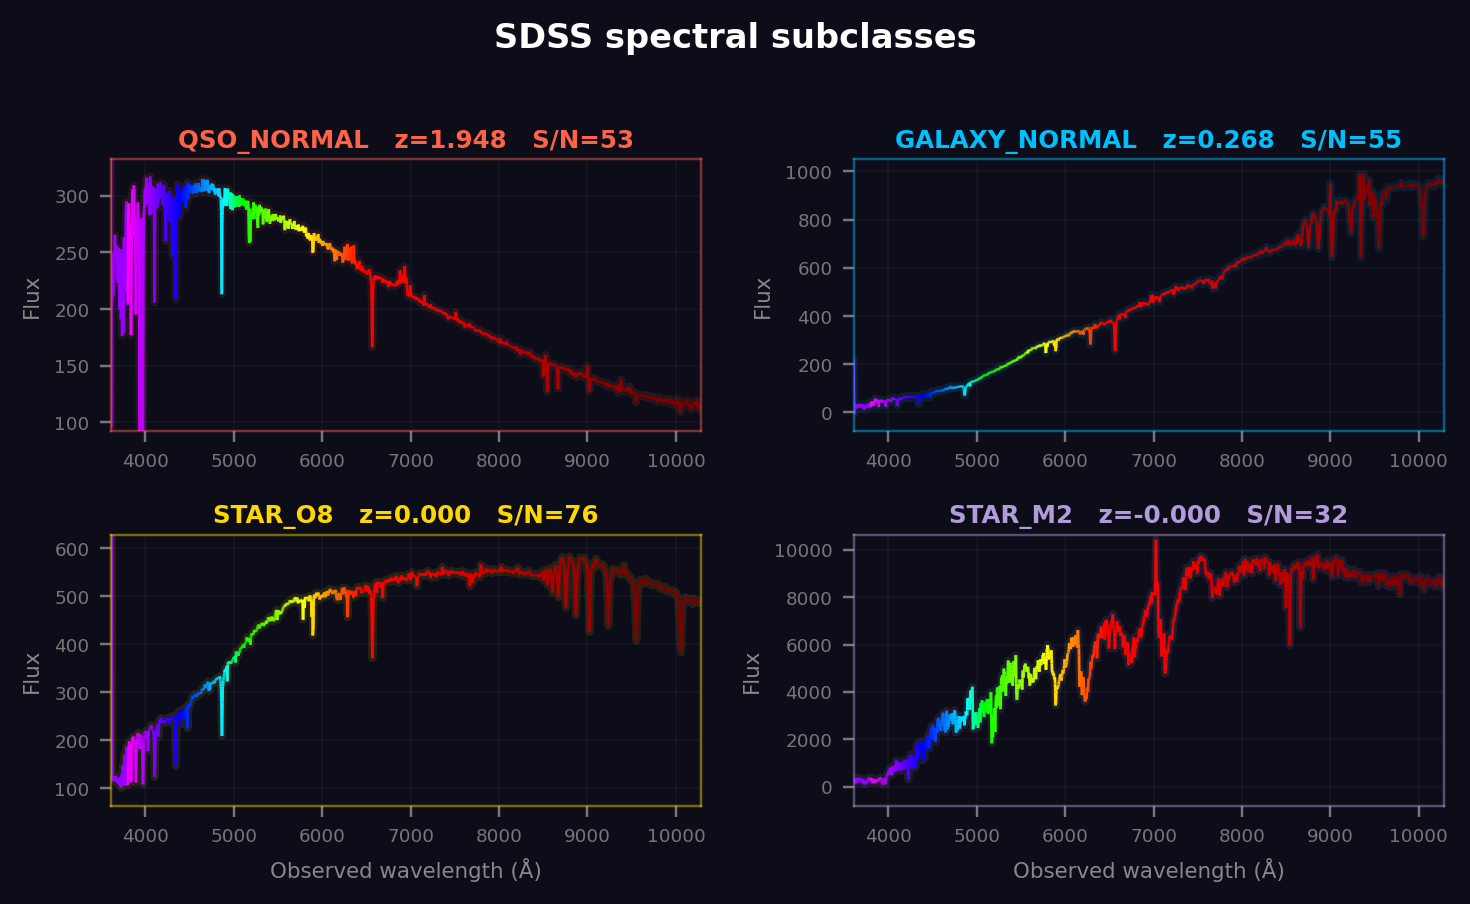
\includegraphics[width=0.95\columnwidth]{Figures/sdss_spectra_example.png}
    \caption{2x2 matrix showcasing examples of four distinct spectral classes from our curated SDSS DR19 dataset. (Classes shown: QSO\_NORMAL, GALAXY\_NORMAL, STAR\_O8, STAR\_M2)}
    \label{fig:spectra_examples}
\end{figure}